\ProvidesFile{ch-light-curve-inversion.tex}[Light Curve Shape Inversion]
\graphicspath{{/Users/liamrobinson/Documents/msthesis/static_images/aas_2022_figs}}
\chapter{Light Curve Shape Inversion}

\section{Direct Inversion}

Traditionally, direct light curve inversion involves two distinct steps: a linear least squares problem to fit an EGI to the measured light curve, and a second optimization to produce accurate vertex positions and face adjacency information \cite{fan2020thesis}. The first step uses data-driven estimation to yield a valid and accurate EGI through a linear optimization. The second step is highly nonlinear and scales badly with facet count and geometric asymmetry, as discussed by Fan in \cite{fan2019}.

\subsection{The Extended Gaussian Image} \label{sec:egi_definition}

The discrete EGI $\vec{E} \in \mathbb{R}^{m \times 3}$ is composed of $m$ unit vectors $\hat{n}$ each scaled a nonnegative scalar $a \in \mathbb{R}, \: a_i \geq 0$ \cite{little1983}.

\begin{equation}
  \vec{E}_i = a_i \hat{n}_i
\end{equation}

In the context of shape inversion, we want to choose the $m$ vectors $\hat{n}$ to be a uniform tessellation on the unit sphere. A convex polytope can be uniquely represented by an EGI of facet normal vectors scaled by each facet's area. The set of normal vectors in an EGI is denoted $\mathcal{N}$ with the set of areas denoted $\mathcal{A}$. The vector of facet areas is denoted $\vec{a} \in \mathbb{R}^{m \times 1}$. In this paper, we take the norm of the EGI to be $\| \vec{E} \| = \vec{a}$ with the `size' of the EGI $\|\vec{E}\| = m$.

The solution to the Minkowski problem proves the existence and uniqueness of a convex polytope for an EGI that satisfies the closure condition in Eq. \ref{egi_closure} \cite{minkowski1909}. Equivalently, an EGI uniquely represents a closed, convex polyhedron --- a polytope --- with no open boundaries, up to a translation.

\begin{equation} \label{egi_closure}
  \sum_{i=1}^m a_i \hat{n}_i = [0, 0, 0]
\end{equation}

While a given EGI uniquely represents a polytope, it is shared by an infinite number of non-convex and open geometries. An example of this extended family is depicted in Figure \ref{fig:egi_family} where larger circles indicate greater relative areas assigned to a given normal vector.

\begin{figure}[!htb]
  \centering
  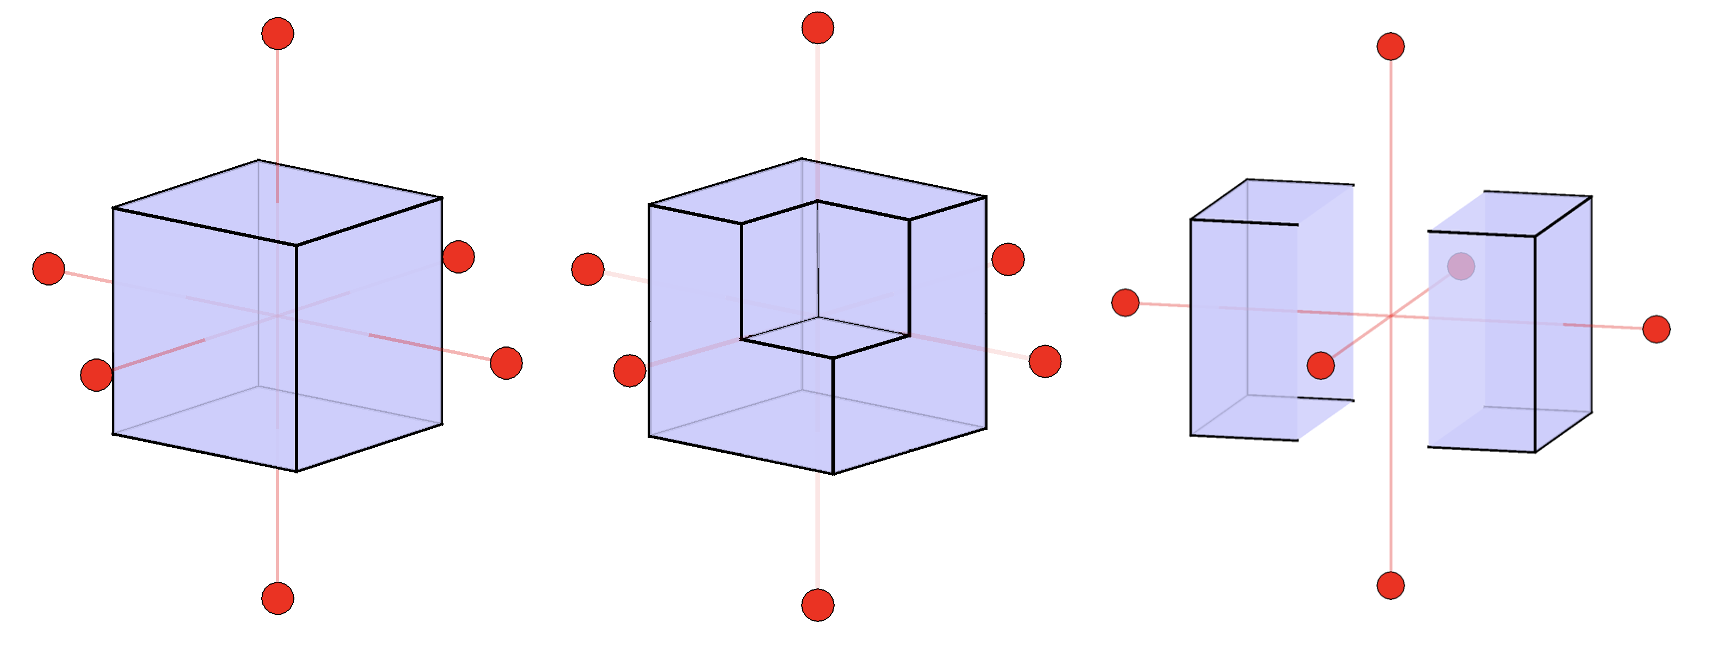
\includegraphics[width=\figmed]{convex_non_open_egis.png}
  \caption{Simplified convex, non-convex, and open EGI nonuniqueness}
  \label{fig:egi_family}
\end{figure}

\subsection{EGI Optimization}

The EGI fulfills two important criteria when applied to light curve inversion: it can be estimated directly from the light curve, attitude profile, and material properties, and uniquely represents a convex object \cite{kaasalainen2001}. Furthermore, convex geometry can be reconstructed from the EGI and vice versa through the dual transform \cite{little1985} and the Minkowski problem \cite{minkowski1909}. 

Once a light curve is obtained, direct shape inversion schemes sample $m$ candidate normal vectors $\hat{n}$ on the unit sphere to fit an EGI to the observed light curve $\vec{L}_\textrm{ref} \in \mathbb{R}^{n \times 1}$ \cite{friedman2020, fan2020thesis}. This is accomplished by solving an optimization problem to distribute the area vector $\vec{a}$ across the sampled normals to minimize the residual between the observed and modeled light curves. In practice, this is a constrained nonnegative least squares problem and can be solved efficiently for large numbers of normal vectors and light curve data points:

\begin{equation} \label{area_opt_convex}
  \min_{a}{\|\vec{L}_{\textrm{ref}} - G \vec{a}\|_2} \:\:\: \textrm{ subject to } \vec{a}_i \geq 0, \: \sum_{i = 1}^{m} \vec{a}_i \hat{n}_i = [0, 0, 0].
\end{equation}

It is important to note that the area estimated with Eq. \ref{area_opt_convex} is necessarily \textit{albedo-area} due to the diffuse reflectivity coefficient $C_d$ in Eq. \ref{lc_func_diffuse}. If the value of $C_d$ is uniform but unknown, the recovered geometry will incorrectly scaled without impacting the face adjacency or relative feature sizes.

The convex reflection matrix $G \in \mathbb{R}^{n \times m}$ with $ij$th entries $[g]_{ij}$ defined at time $i$ for each facet $j$ is defined as the normalized received facet irradiance per unit facet area:

\begin{equation} \label{ref_cond_matrix}
  [g]_{ij} = \frac{I_{ij}}{I_\textrm{Sun} a_j}.
\end{equation}

This relationship between the object irradiance and area defines the normalized convex light curve $\vec{L}_{\textrm{convex}}$, that produced by a convex object of facet areas $\vec{a}$ under the attitude profile and lighting conditions that yield $G$.

\begin{equation} \label{convex_lc_with_g}
  \vec{L}_{\textrm{convex}} = G \vec{a}
\end{equation}

\subsection{EGI Optimization Results}

The optimization in Eq. \ref{area_opt_convex} produces a coarse approximation of the true EGI as $m$ is finite. Increasing $m$ necessarily improves the quality and sparsity of the estimated EGI, but at the cost of computational resources. The estimation was performed using a synthetic light curve input from $n=500$ Sun and observer vectors uniformly sampled on the sphere in the body frame, producing a full rank $G$ matrix. $m = 500$ candidate normal vectors were sampled using a spherical Fibbonaci mapping described by Keinert et al. in \cite{keinert2015}. Results are visualized for an icosahedron in the body frame in Figure \ref{initial_ico_resampling}. Reconstructing the object at this stage is difficult due to the quantity of faces present in the estimated EGI. 

\begin{figure}[!htb]
  \centering
  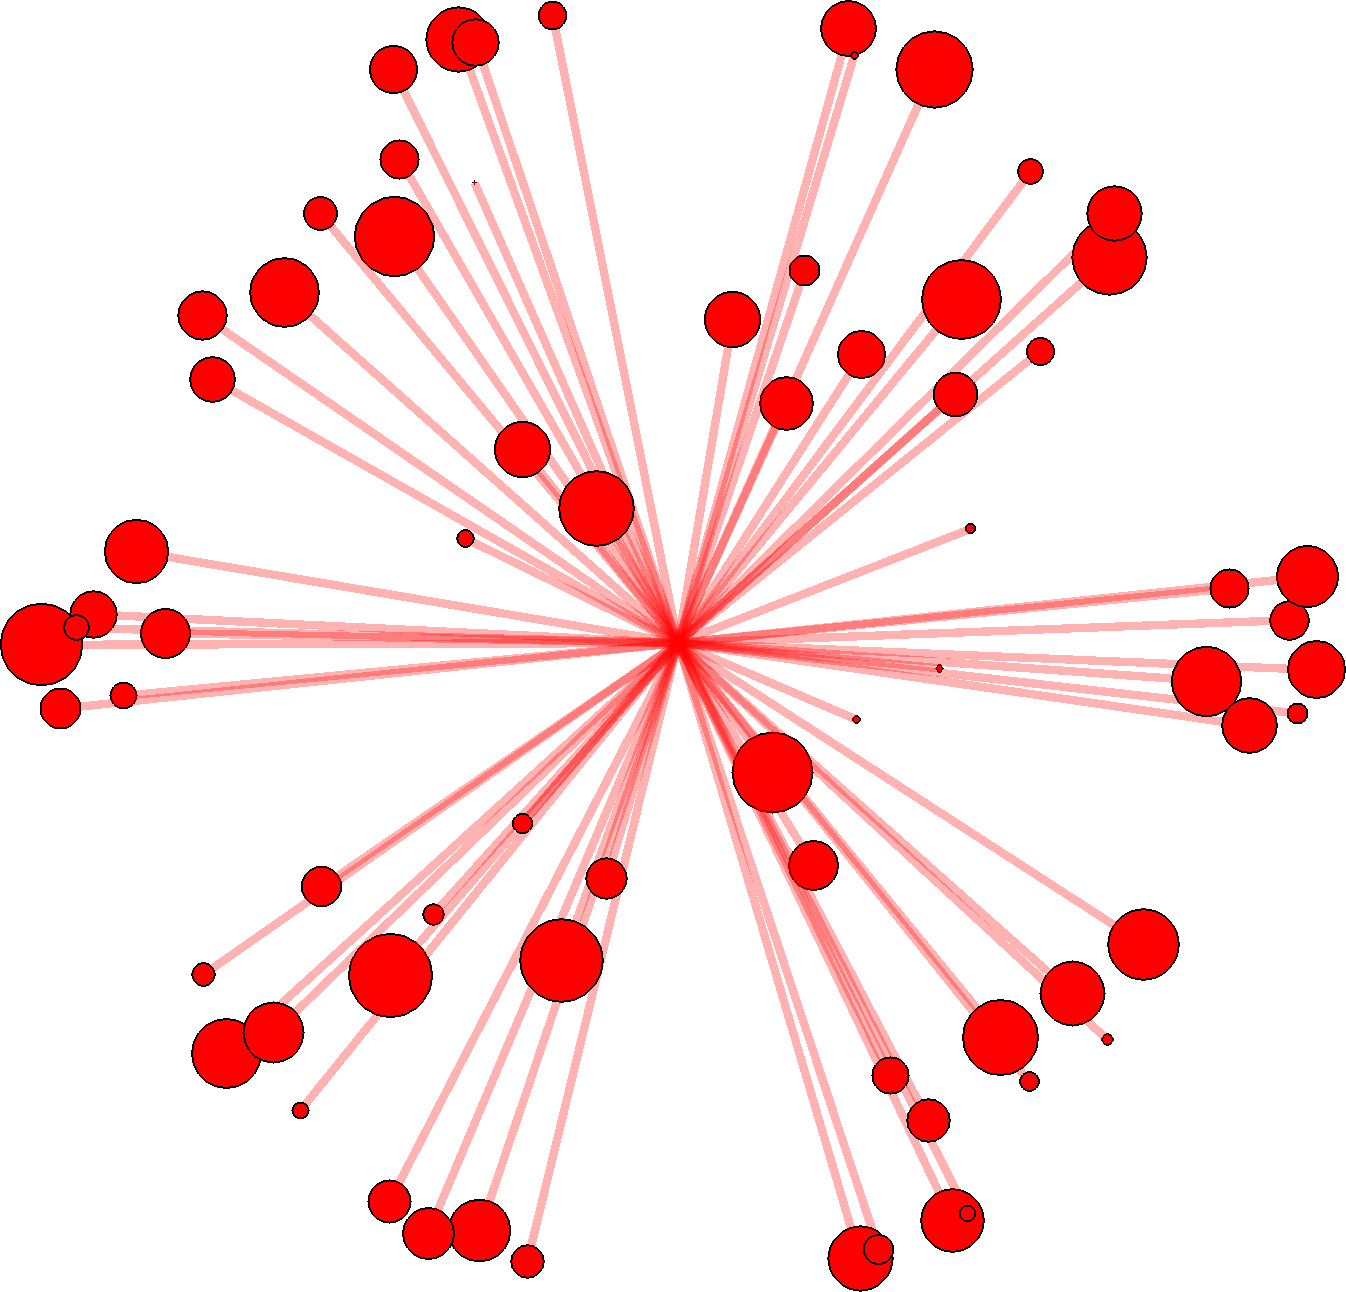
\includegraphics[width=150px]{ico_initial_egi.png}
  \caption{Initial icosahedron EGI optimization before resampling}
  \label{initial_ico_resampling}
\end{figure}

\subsection{EGI Resampling}

We propose a normal vector resampling step to promote a more accurate and sparse EGI. The normal vectors used in Eq. \ref{initial_ico_resampling} are generally correct, with each group clustering around a normal vector of the truth geometry. This clustering behavior occurs when none of the candidate normal vectors are sufficiently close to the truth. Resampling in a cone centered on each initial EGI normal vector provides more accurate candidates for EGI estimation. This process mimics a single optimization step with a much larger $m$, where the coarse EGI is used to exclude areas on the sphere with little or no normal area.

Uniformly sampling a cone of half-angle $\phi$ is accomplished by strategically sampling points on the unit sphere. 

\begin{equation} \label{cone_sample_n_pole}
  \hat{n}_{cone} = \begin{bmatrix}
    \sqrt{1-z^2}\cos{\theta} \\
    \sqrt{1-z^2}\sin{\theta} \\
    z \\
  \end{bmatrix}
\end{equation}

In Eq. \ref{cone_sample_n_pole} we choose two coordinates $z \in [\cos{\phi}, 1]$ and $\theta \in [0, 2\pi)$, yielding a point uniformly distributed on a cone of half-angle $\phi$ about the central axis $[0, 0, 1]^T$ \cite{cone_sampling_wolfram}. These points are then rotated using a direction cosine matrix to center the cone on an axis of interest.

The number of new candidates sampled per initial solution vector and the cone half-angle should be adjusted on a case-by-case basis depending on the compute power available and light curve data quality.

\subsection{EGI Resampling Results}

Existing EGI optimization schemes like those of Fan \cite{fan2020thesis}, Friedman \cite{friedman2020}, and Cabrera \cite{cabrera2021} are limited by a single normal vector sampling step, leading to a lack of accuracy and sparsity in the optimized EGI. High-density normal vector sampling in regions known to contain non-zero area leads to EGI solutions that are generally more sparse and cluster more tightly about true normal vectors.

This process is shown in Figure \ref{resampled_ico_ns} for the same icosahedron with a half-angle $\phi = \frac{\pi}{20}$ and sampling density of $50$ candidate vectors per cone.

\begin{figure}[!htb]
  \centering
  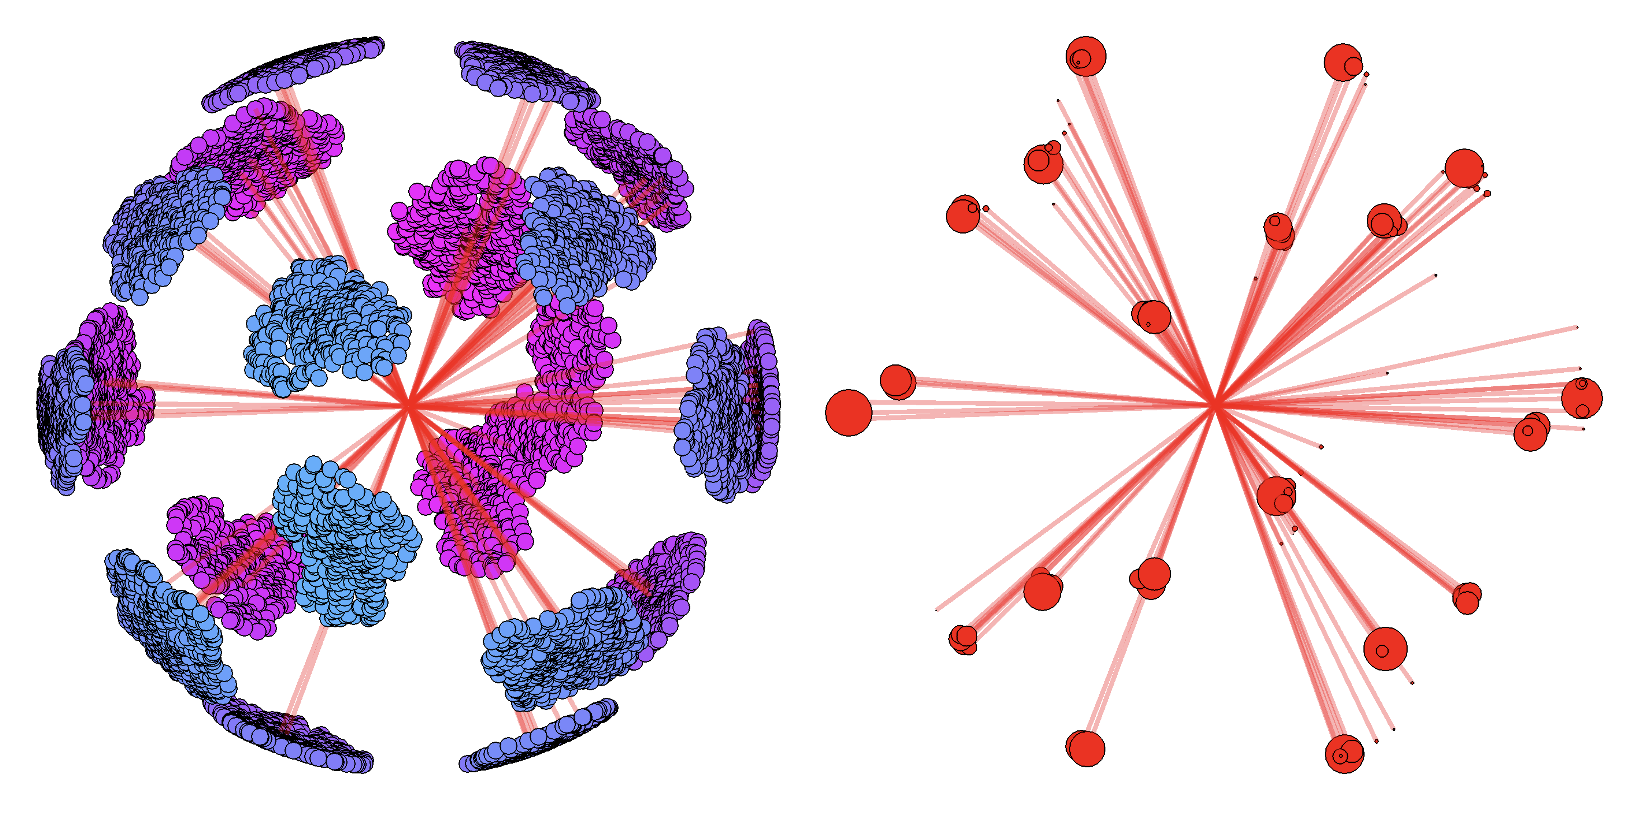
\includegraphics[width=350px]{ico_resampled_with_flower.png}
  \caption{Resampled normal vectors (left) with reoptimized EGI (right)}
  \label{resampled_ico_ns}
\end{figure}

\subsection{EGI Merging}

After resampling and reoptimizing with Eq. \ref{area_opt_convex}, the reestimated EGI is merged by computing all groups $\mathcal{G}$ of EGI vectors within an angular offset $\alpha$:

\begin{equation}
  \mathcal{G}_k = \left\{ \vec{E}_i \in \vec{E} \:\| \cos^{-1}\left( \frac{\hat{E}_i \cdot \hat{E}_k}{\|\vec{E}_i \| \| \vec{E}_k \|}\right) < \alpha \right\}.
\end{equation}

Groups are merged by summing all group members, yielding a single EGI vector $\vec{E}_m$ without loss of total area or closure. 

\begin{equation} \label{eq:fixing_egi}
  \vec{E}_m = \sum_{\vec{E} \in \mathcal{G}_k}{\vec{E}}
\end{equation}

In practice, the choice of $\alpha$ is dependent on the user's tolerance for discretization, as merging will approximate smooth geometry by discrete faces with normal vectors offset by $2\alpha$.

\subsection{EGI Merging Results}

Merging the resampled EGI using Figure \ref{resampled_ico_ns} with $\alpha = \frac{\pi}{10}$ produces a final sparse EGI fit for object reconstruction, shown in Figure \ref{ico_merged_egi}. 

\begin{figure}[!htb]
  \centering
  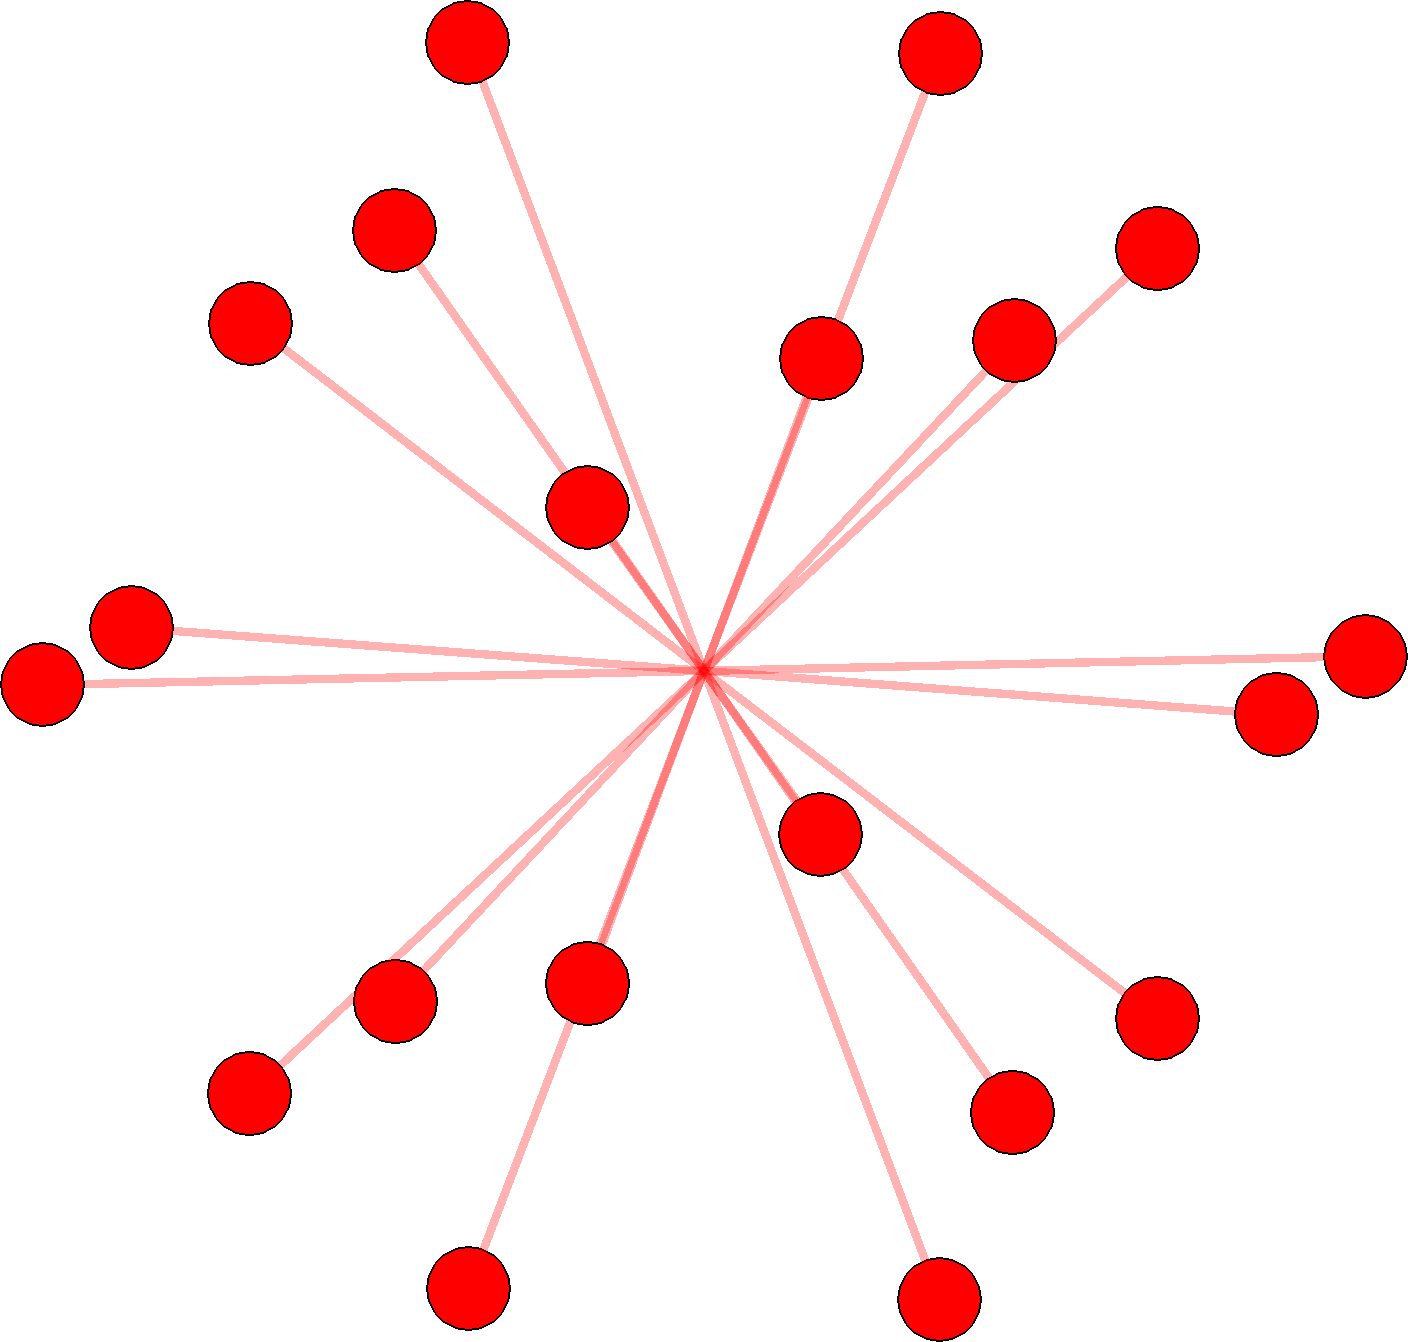
\includegraphics[width=150px]{ico_merged_egi.png}
  \caption{Merged icosahedron EGI}
  \label{ico_merged_egi}
\end{figure}

\subsection{Convex Geometry Recovery from the EGI}

At this stage, we have recovered a sparse EGI representing a convex approximation of the underlying object with no guarantee of the closure of this EGI. The EGI closure constraint Eq. \ref{egi_closure} motivates a simple procedure to correct an invalid EGI by adding the mean closure error to each entry:

\begin{equation} \label{egi_validation}
  \vec{E}_{\textrm{closed}} = \vec{E}_{\textrm{open}} - \sum_{i=1}^m a_i \hat{n}_i .
\end{equation}

This step is not a novel contribution. Fan used a more complex optimization problem to adjust the EGI towards closure \cite{fan2020thesis}. We improve on that process with a simpler analytical correction. In practice, this process should be performed before each reconstruction to accelerate convergence. Failing to correct non-closed EGIs will cause convergence to a nonzero minimum in the reconstruction objective function as there is no corresponding convex object with the given EGI.

The unique convex object encoded by each closed EGI is reconstructed by solving for the polytope's set of vertices $\mathcal{V}$ and faces $\mathcal{F}$ encoding the adjacency relations between vertices. This is accomplished following the procedure introduced by Little in \cite{little1983} through the dual transformation. The dual set $\mathcal{D}$ are vertices in $(A, B, C) \in \mathbb{R}^3$ that satisfy the following plane condition for a point $(x, y, z)$ on each facet of the object:

\begin{equation} \label{dual_abc_form}
  Ax + By + Cz + 1 = 0
\end{equation}

If $(x, y, z)$ are chosen to be the closest points in the object's planes to the origin, the dual set $\mathcal{D}$ can be expressed in terms of the EGI and a support vector $\vec{h} \in \mathbb{R}^{\|F\| \times 1}$. The support vector is the perpendicular distance of each facet defining the object to the origin.

\begin{equation} \label{dual_egi_form}
  \mathcal{D} = \frac{\vec{E}}{ \| \vec{E} \| \vec{h}}
\end{equation}

The object's vertices $\vec{v}_{ref}$ are found by computing the convex hull of dual set vertices. Triplet of vertices on the resulting faces are used to find a single real vertex by intersecting the three planes defining the dual set vertices.

\begin{equation}
  \begin{bmatrix}
    v_{ref,x} \\
    v_{ref,Y} \\
    v_{ref,Z} \\
  \end{bmatrix} = \begin{bmatrix}
    v_{i,x} & v_{j,x} & v_{k,x} \\
    v_{i,y} & v_{j,y} & v_{k,y} \\
    v_{i,z} & v_{j,z} & v_{k,z}
  \end{bmatrix}^{-1} \begin{bmatrix}
    1 \\ 1 \\ 1
  \end{bmatrix}
\end{equation}

Convex face adjacency information is found by triangulating the convex hull of all reference vertices. The accuracy of the recovered geometry is entirely dependent on the correctness support vector $\vec{h}$ used to produce the dual set. Finding the true support vector is the challenge of the final optimization in convex shape inversion.

\subsection{Support Vector Optimization}

Prior work by Fan used Little's objective function for support vector optimization \cite{fan2020thesis,little1983}.

\begin{equation} \label{little_obj}
  f(\vec{h})_{\textrm{Little}} = \vec{h} \cdot \vec{a}
\end{equation} 

TODO

\section{Non-Convex Feature Inversion}

\subsection{Non-Convex Feature Detection and Location}

Many human-made space objects are, as highlighted in Figure \ref{hst_bennu_shadows}, highly non-convex. As a result, their shape inversion is plagued by the fact that the Minkowski problem-driven reconstruction methods of Eq \ref{little_problem} cannot recover non-convex features. Instead of beginning from the ground up, we can leverage the convex shape guess to detect and locate concavities, if they are present.

We can retain information about large, unilateral object concavities during  EGI estimation in Eq. \ref{area_opt_convex} by relaxing the EGI closure constraint. This unconstrained form is also generally functional for most convex objects and can be used without loss of detail in the final reconstruction as long as closure correction in Eq. \ref{eq:fixing_egi} is still employed.

By measuring the divergence of the optimized EGI from a closed object with the magnitude of the closure error $\vec{e}_{EGI}$, we can determine the mean axis of prominent concave features.

\begin{equation} \label{eq:closure_error}
  \vec{e}_{EGI} = -\sum_{i=1}^{m} a_i \hat{n}_i.
\end{equation}

This EGI closure error vector represents the missing area on each body axis that could be added to close the object. The addition of the minus sign transforms the vector from expressing the presence of excess area to the absence of missing area. The closure error will be negligable if there are no concavities present. The closure error may also be negligable if there is no self-shadowing is present over the sampled attitude profile, therefore the closure error merely quantifies the self-shadowing that is occuring, not whether there may be self-shadowing in other orientations.

Under the strong assumption that the concavities present are major and unilateral, this EGI error vector points along the mean axis of the concavity.

After locating the concave feature through the direction of the EGI error vector, the magnitude of the same vector is used to recover a more accurate non-convex guess for the object geometry. We have found that the $\ell^2$-norm of the EGI error vector --- the total missing area required to close the object --- scales quadratically with object scale. A quadratic relationship is expected as geometrically scaling vertex positions by a factor $c$ increases object area by a factor $c^2$, leading to an identical light curve and estimated EGI with $c^2$ as much area assigned to each facet, scaling $\vec{e}_{EGI}$ identically. 

It can also be shown that for simple, unilateral concave features, the internal angle $\psi$ between shadowing faces scales linearly with the quantity $\sqrt{\frac{\|\vec{e}_{EGI}\|}{\|\vec{E}_{m}\|}}$ where $\vec{E}_m$ is the estimated EGI after merging. We can estimate the internal angle as a function of the optimized EGI, its error, and an unknown slope $c$.

\begin{equation} \label{eq:internal_angle_eq}
  \psi = \pi - c \sqrt{\frac{\|\vec{e}_{EGI}\|}{\|\vec{E}_{m}\|}}
\end{equation} 

This relationship is displayed in Figure \ref{combined_error_relationship} for two different object geometries, each with prominent and unilateral concavities.

\subsection{Concavity Location Results}

The slope $c$ has been shown through simulation to be independent of object geometry, with $c=8$ being highly accurate for a majority of simulated objects with large and unilateral concavities, resulting from an interaction between the shadowing geometry and the least squares EGI optimization. This solution is not unique \cite{durech2003}, and is best interpreted as finding the simplest non-convex object that would result in the same EGI closure error vector.

\begin{figure}[!htb]
  \centering
  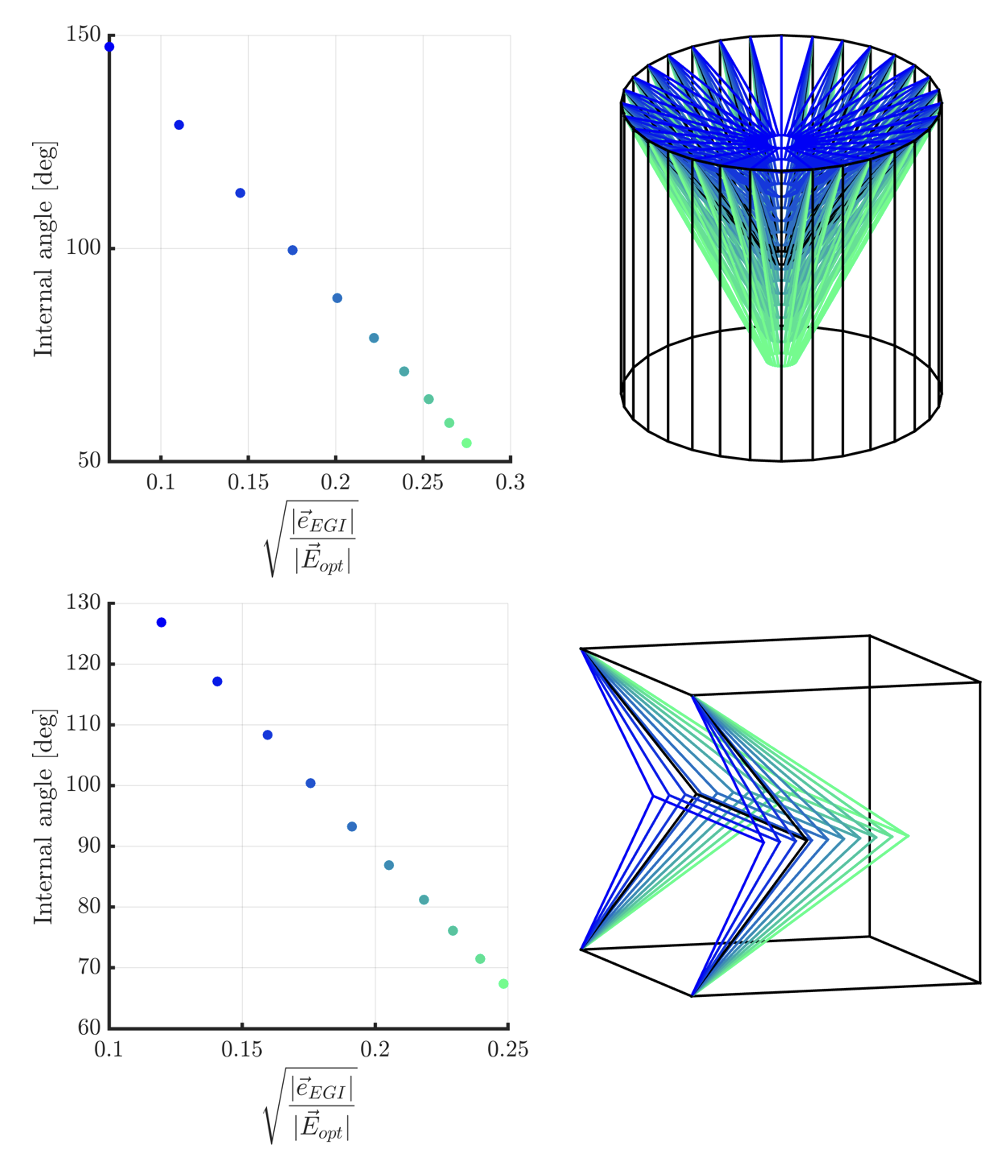
\includegraphics[width=250px]{error_mag_study/combined_error_mag.png}
  \caption{Concave cylinder and house EGI error relationship to internal angle}
  \label{fig:combined_error_relationship}
\end{figure}

\subsection{Concavity Creation}

Our process for creating an accurate concavity in the reconstructed convex guess proceeds in four major steps. The model is first subdivided to add more faces and vertices. Subdivided vertices are then classified by their proximity to the EGI error vector, indicating whether their positions should be updated. Boundary vertices are identified, and vertex positions are updated based on the estimated internal angle computed via Eq. \ref{eq:internal_angle_eq}.

\subsubsection{Model Subdivision}

Subdividing the initial convex object guess is essential for retaining object detail during concavity creation. We use a combination of geometry processing algorithms for linear subdivision, Loop subdivision, and remeshing. Linear subdivision is advantageous when object faces are equally sized and boundary edges must be maintained. Loop subdivision is preferable when there are numerous vertices so that subdivisions do not drastically diverge from the initial boundary surface. Loop subdivision softens sharp edges as it relies on B-splines to interpolate new vertex positions \cite{loop1987}. The specific type and resolution of subdivision used depends on the level of detail the user needs to maintain in the introduced concavity, although linear subdivision followed by Loop subdivision is a useful baseline. Varying combinations of subdivision are shown in Figure \ref{fig:subd_grid} to illustrate the available configurations.

\begin{figure}[!htb]
  \centering
  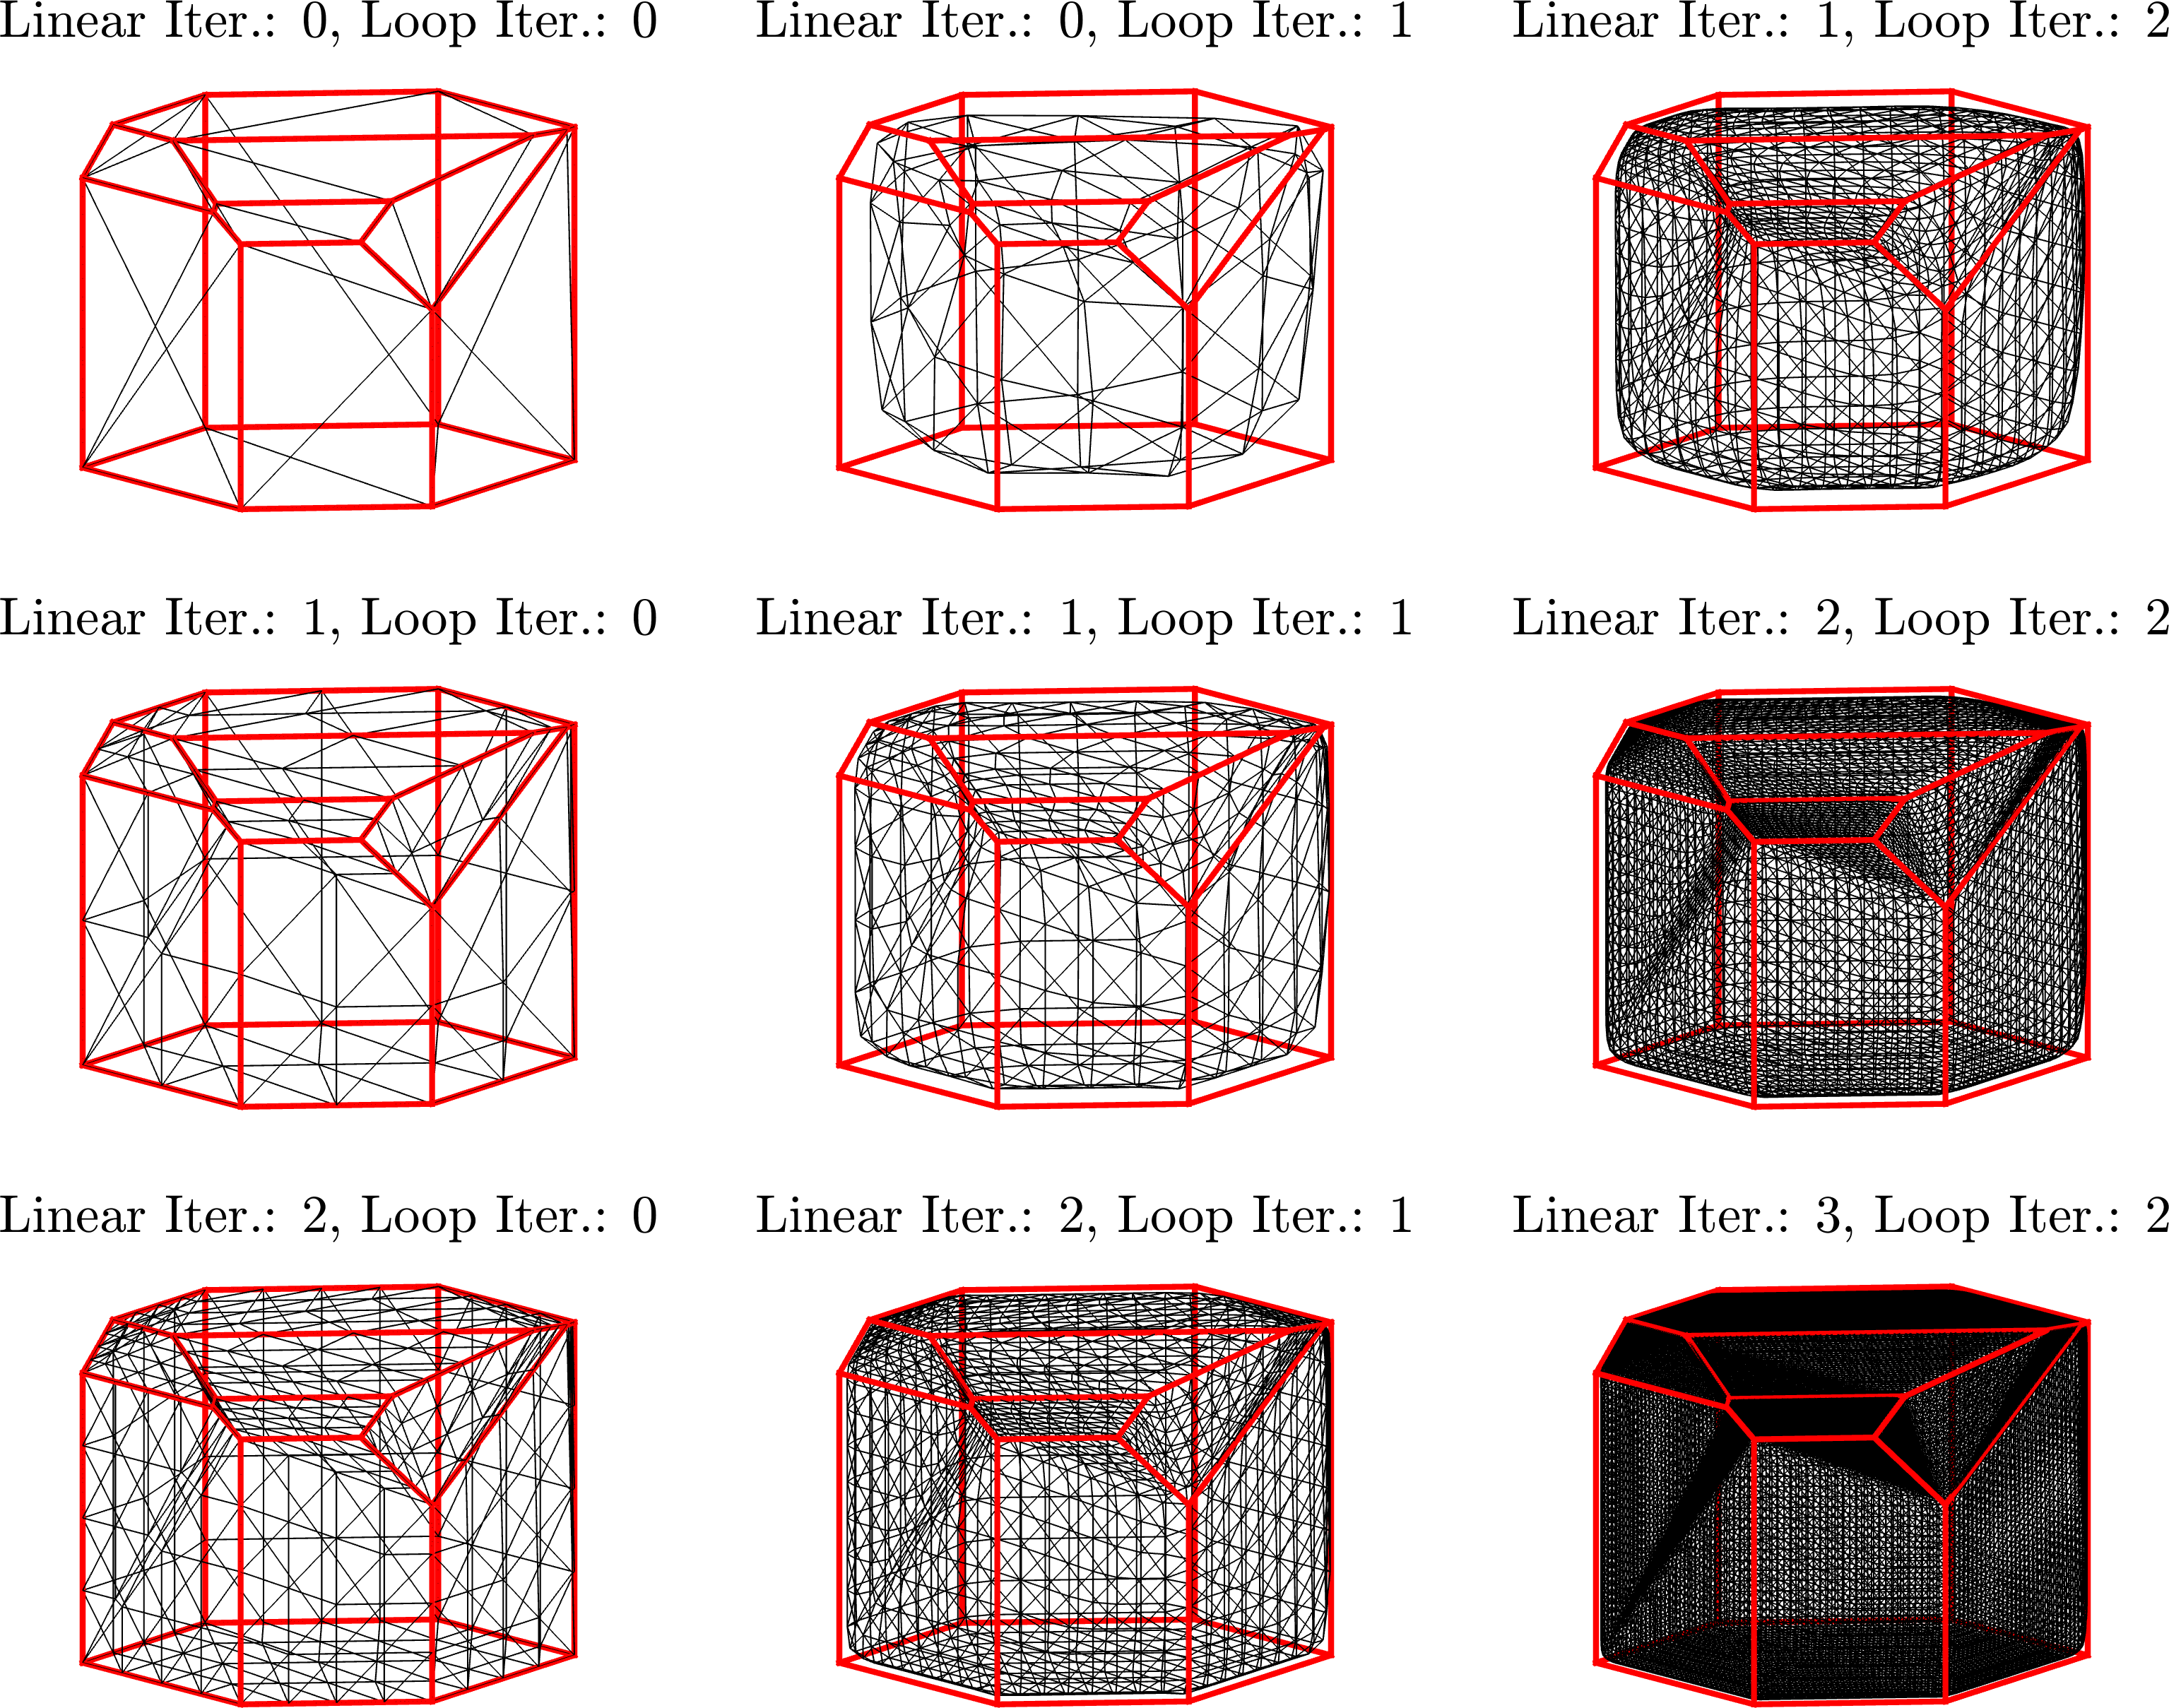
\includegraphics[width=350px]{subd_grid.png}
  \caption{Subdivided object (black) with reference (red) with various levels of subdivision}
  \label{fig:subd_grid}
\end{figure}

\subsubsection{Vertex Classification}

When introducing a concavity, it is important to classify which vertices are part of the concave feature --- and therefore need to be updated --- and which vertices should remain unaffected. This is accomplished by measuring the angle from each face normal to the EGI error vector, where faces with normal vectors within an angle of $\pi/2$ to the error vector must be updated. In reality, all face normals and areas are impacted by the presence of the concavity in the area optimization Eq. \ref{area_opt_convex} and EGI correction step Eq. \ref{egi_validation}. We select the angle deflect $\pi/2$ to update all faces above the horizon from the EGI error vector, a bound which tends to produce visually accurate concavities. Faces requiring an update are termed \textit{free} faces, with all others termed \textit{root} faces.

\subsubsection{Vertex Displacement}

For all vertices on free faces, we can further distinguish \textit{root-adjacent} and \textit{free} vertices. Root-adjacent vertices are part of at least one root face, whereas free vertices belong to only free faces. Classifying vertices in this way results in a border of root-adjacent vertices around the interior free vertices, visualized in Figure \ref{fig:root_and_free}.

\begin{figure}[!htb]
  \centering
  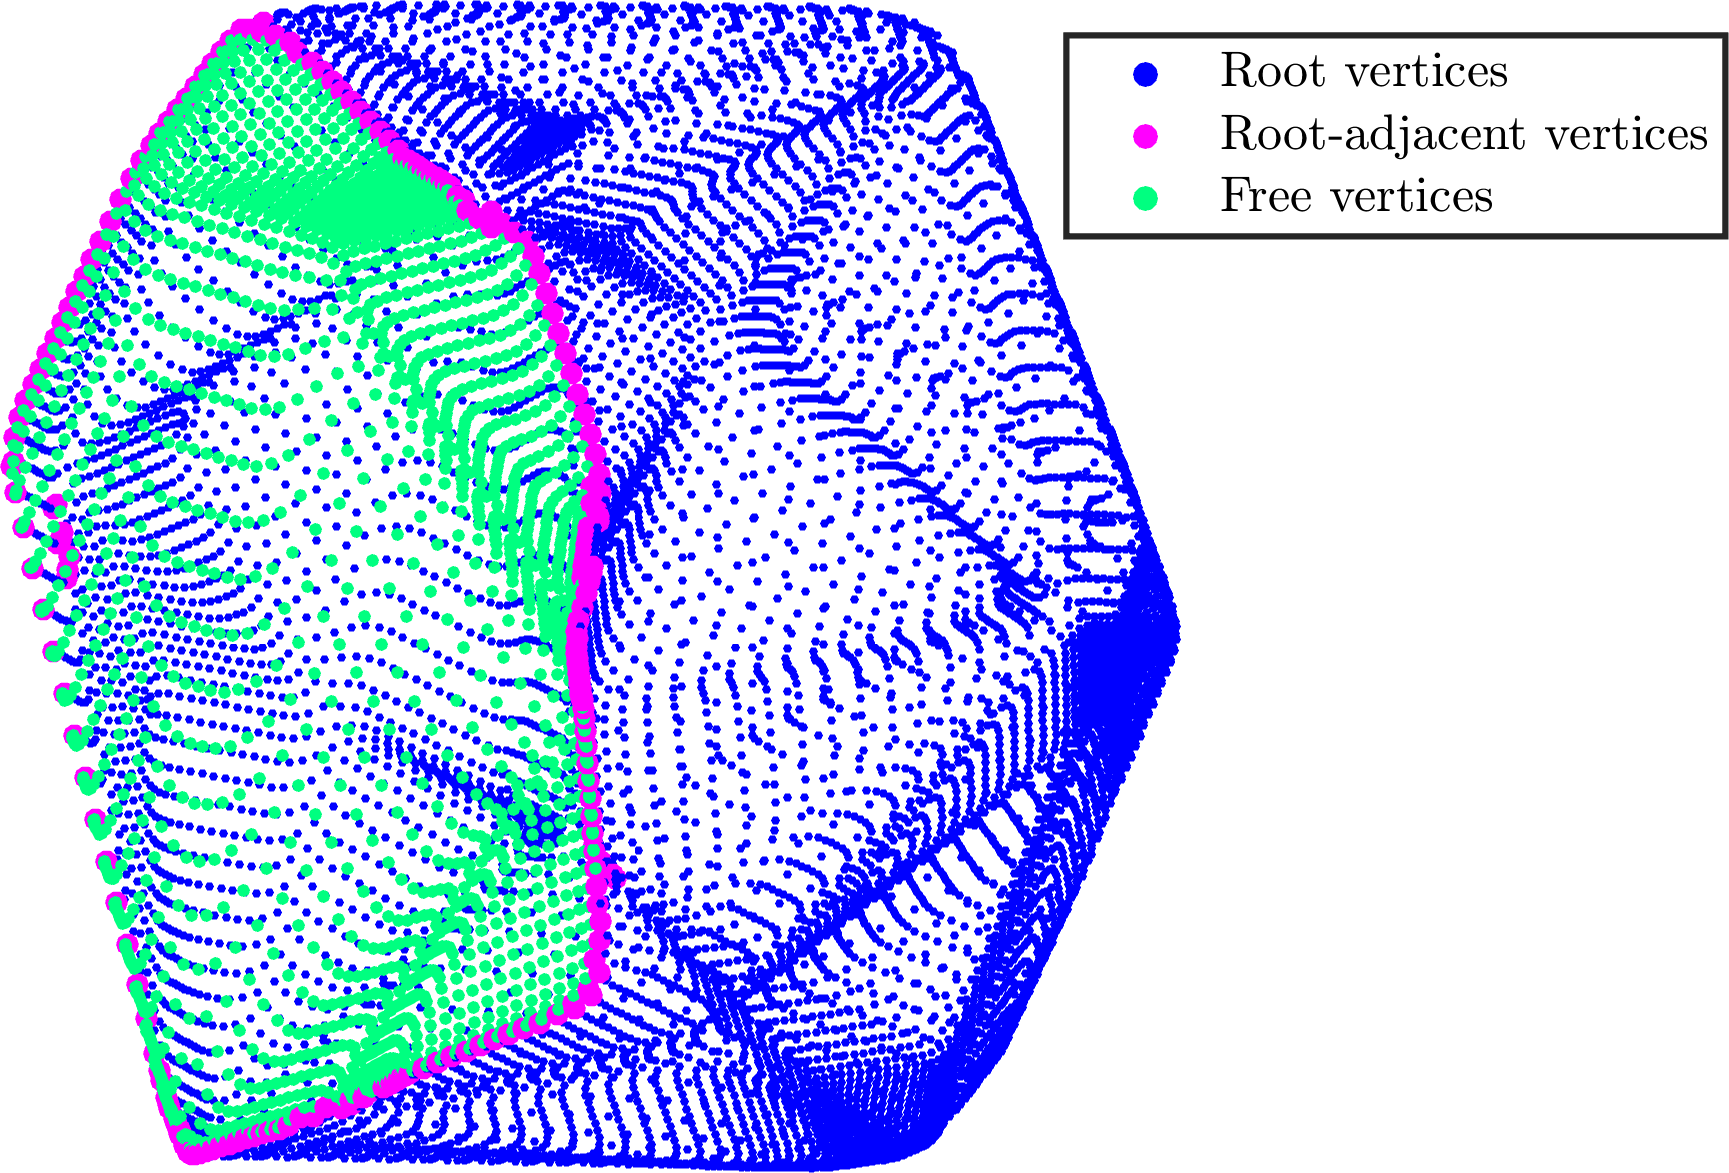
\includegraphics[width=250px]{rootadj_and_free_verts_try2.png}
  \caption{Root-adjacent and free vertices}
  \label{fig:root_and_free}
\end{figure}

Given the estimated internal angle $\psi_{est}$ and the error vector $\hat{e}_{EGI}$, each $i$th free vertex is displaced to introduce a geometrically accurate concavity by moving each a distance $d_i$ in the direction of $-\hat{e}_{EGI}$:

\begin{equation} \label{eq:flip_depth}
  d_i = p_i \sqrt{\csc^2 \frac{\psi_{est}}{2} - 1},
\end{equation}

where $p_i$ is the distance from each $i$th free vertex to the nearest root-adjacent vertex.

\section{Non-Convex Object Reconstruction Results}

Displacing free vertices in the EGI error vector direction by $d_i$ yields accurate concavities for objects whose concave boundaries lie in a plane. The result of applying this process to a set of representative convex objects is shown in Figure \ref{fig:non_convex_recon_of_non_convex} using the same attitude profiles and as in Figure \ref{convex_grid}. 

\begin{figure}[!htb]
  \centering
  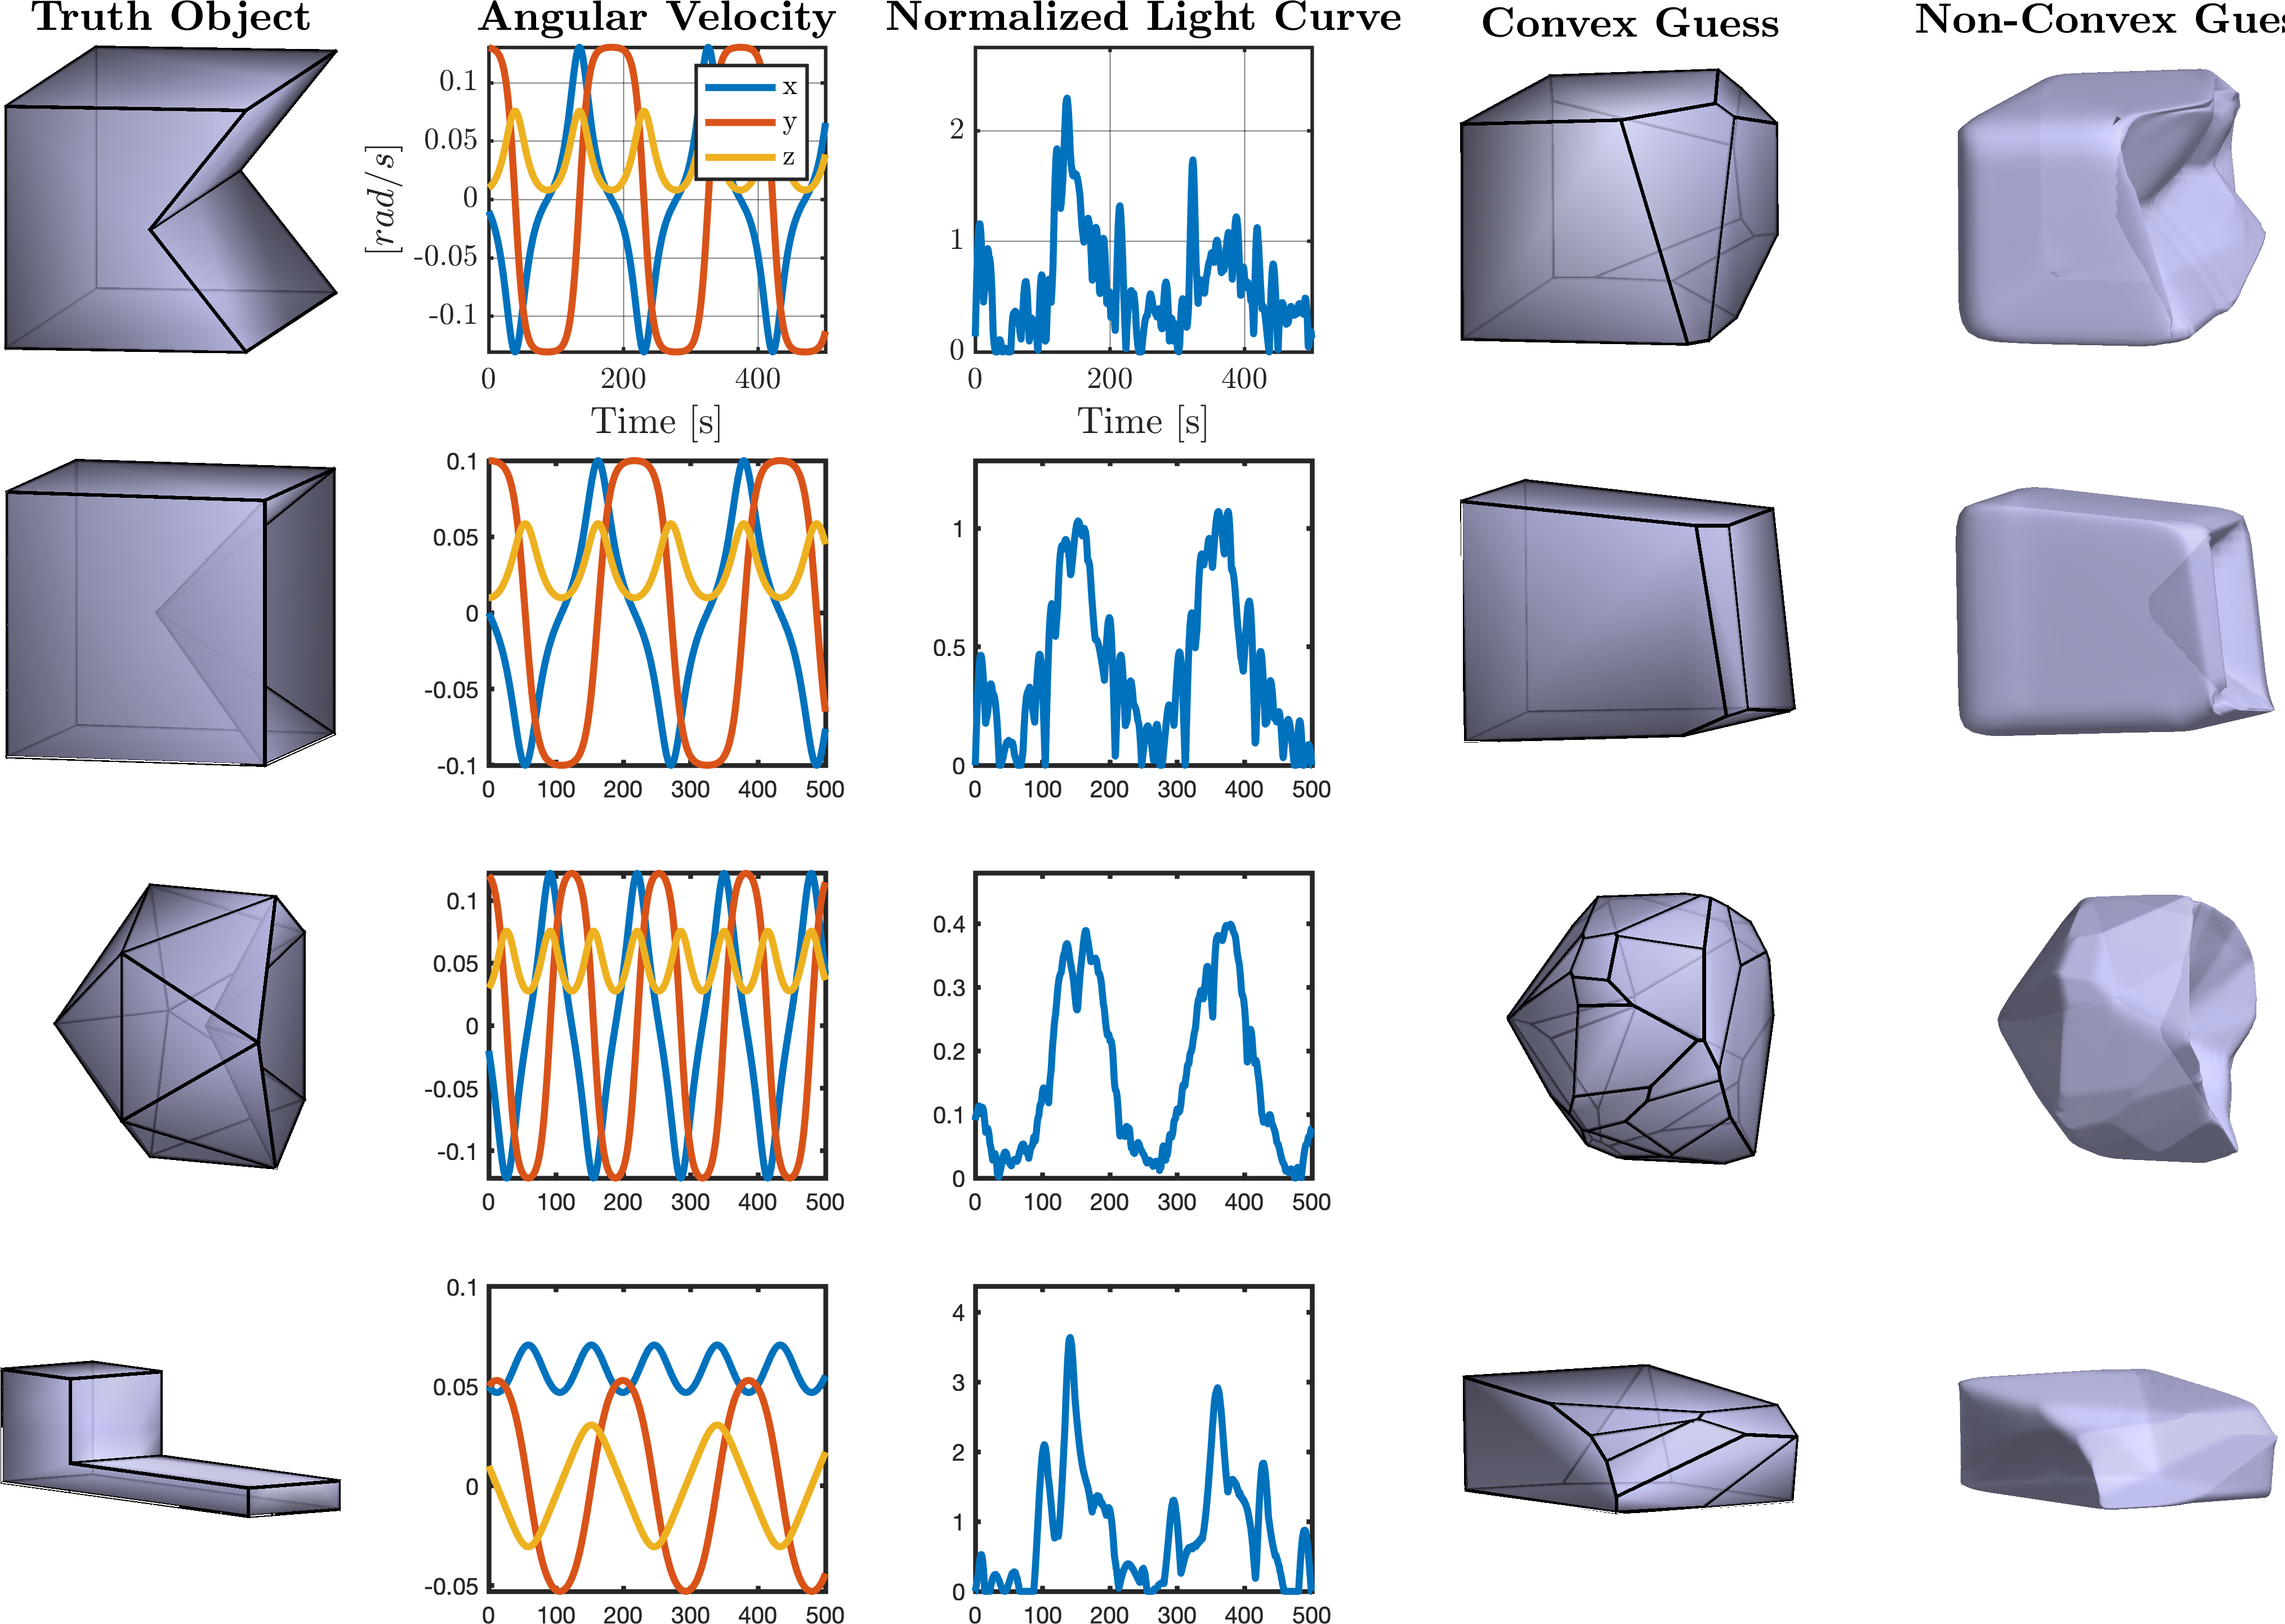
\includegraphics[width=400px]{rec_non_convex_objs/non_convex_grid_of_nonconvex_try2.png}
  \caption{Collapsed house, cube, icosahedron, and box-wing satellite reconstructions using vertex displacement}
  \label{fig:non_convex_recon_of_non_convex}
\end{figure}

The collapsed cube and icosahedron in Figure \ref{fig:non_convex_recon_of_non_convex} are recovered effectively, but the collapsed house and box-wing satellite expose two limitations of the vertex displacement technique. In the case of the house where the concavity boundary is not constrained to a plane, the edges of the created concave feature are incorrect. The box-wing satellite's shadowing geometry leads the convex guess to be a poor approximation of the geometry outside of the concavity while also inheriting the same problem as the house.

This vertex displacement scheme will negligibly impact the convex guess if the truth object is also convex. A convex truth object will produce a small $\|\vec{e}_{EGI}\|$, causing the vertex update depth $d_{i}$ to trend towards zero as the estimated internal angle approaches $\psi = 180^\circ$. This is illustrated in Figure \ref{fig:non_convex_recon_of_convex} using the same input convex objects and attitude profiles as in Figure \ref{convex_grid}.

\begin{figure}[!htb]
  \centering
  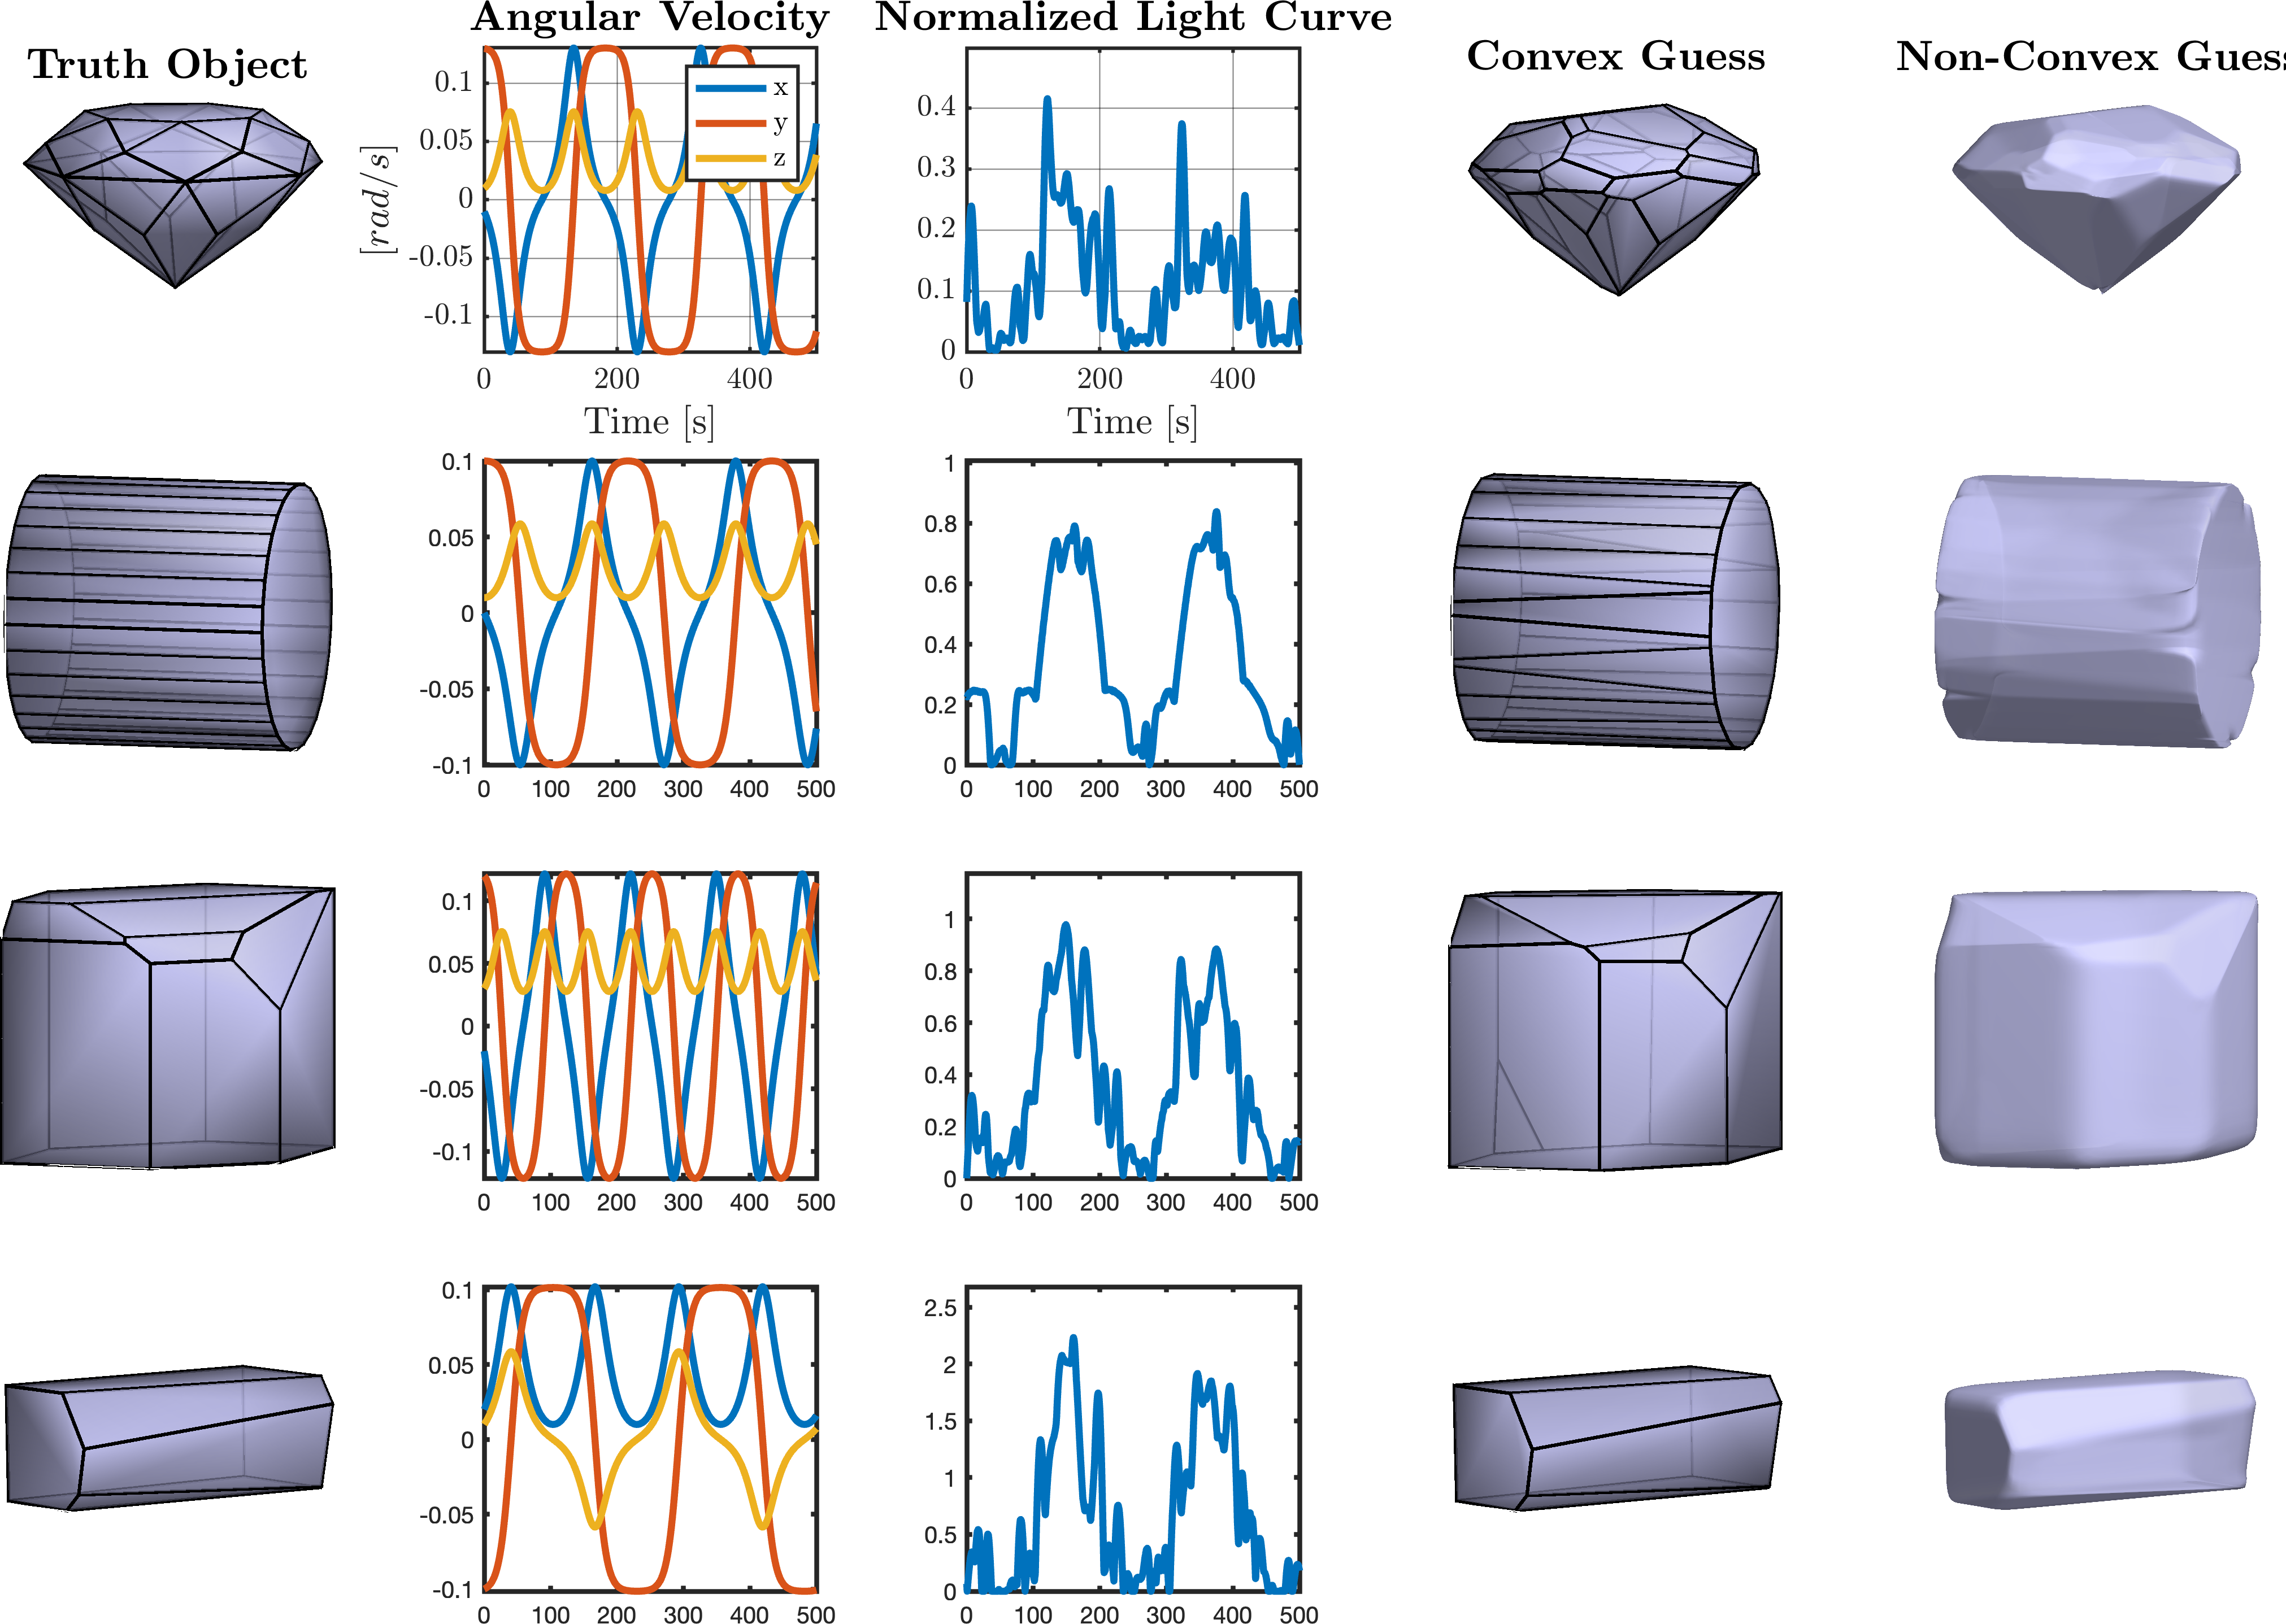
\includegraphics[width=400px]{rec_non_convex_objs/non_convex_grid_of_convex_try2.png}
  \caption{Convex objects under vertex displacement procedure}
  \label{fig:non_convex_recon_of_convex}
\end{figure}

Figure \ref{fig:non_convex_recon_of_convex} clearly displays the compatibility of vertex displacement with truly convex objects. All objects are reconstructed faithfully in both their convex and non-convex inversions, with the same caveats noted in the discussion following Figure \ref{convex_grid}. Some truly sharp edges are rounded during mesh subdivision as seen in the gem or rectangular prism. That said, others like the cylinder become more accurate as subdivision reintroduces continuity lost to discretization in EGI merging.
